% !TEX root = ../thesis.tex
\chapter{弱标注分割蒙版输入下的移动端实时抠图方法}
\section{引言}
上一章中提出了基于相似性学习的信息传播在一般性的图像抠图任务上的应用方法,在本章中我们将研究如何将引导滤波器的思想方法结合到神经网络中,以达到近似引导上下文注意力机制的效果,实现移动端的高效实时抠图。

图像抠图任务的提出不仅仅是为了进行高精度的图像分割,更是为了对自然图像进行合理地分解,因为抠图任务同时需要考虑物体的透明度。抠图算法生成的alpha遮罩可以大大减少广告、设计、电影等行业中对图像或视频进行编辑的工作量以及技能要求。
随着在移动设备上编辑图像或视频的用户数量快速增长,高效、准确且能提升用户体验的自然图像抠图算法已成为一个重要的需求。

目前在移动设备上进行图像抠图存在两个难点。一方面,因为图像抠图是对高分辨率alpha遮罩进行估计的计算密集型任务,目前绝大多数抠图方法\cite{levin2008closed,chen2013knn,cho2016natural,xu2017deep}无法在移动设备上实现实时处理。另一方面,多数现有的抠图方法对输入的trimap图的质量十分敏感。虽然有部分基于涂抹(scribble-based)\cite{lee2011nonlocal}和交互式\cite{yang2018active}的抠图方法在近几年被提出,但是不正确的涂抹或输入信息依然会导致具有复杂纹理的图像的抠图结果存在大量错误。

通常情况下,由于时间延迟和计算能力的限制,我们只能在移动设备上获得弱标注分割蒙版(weakly annotated mask)。我们通过弱标注分割蒙版这个词来描述一个存在噪声或不完全正确的分割蒙版,该蒙版可以对图像上的前景和背景提供一个近似准确的标注信息。这里对弱标注的定义与弱监督分割\cite{papandreou2015weakly}或定位\cite{oquab2015object}中的弱标注略有区别。
弱标注分割蒙版可以是分割方法所输出的二进制图像、阈值化后的深度图或是来自用户交互的不准确的蒙版标注。它与传统的trimap图不同,传统的trimap图是绝对正确的,但需要更多的人工标注时间。
  换句话说,传统的trimap图中要求不存在将前景区域标注为背景的错误情况,或是将部分背景像素标注为前景的错误。大多数传统的图像抠图方法都将输入的trimap图视为完全正确的指导标准,仅在标注的未知区域中计算alpha遮罩值。尽管弱标注分割蒙版意味着在输入的蒙版中会存在此类标注错误,但是如果该蒙版是通过分割方法自动生成的,则此类错误往往无法避免。同时,降低输入trimap图或蒙版的标注质量可能会严重影响传统抠图方法的性能。

先验信息作为对可行域的一个约束,已经在一些先前的工作中被深入研究,以改进图像生成类任务\cite{ulyanov2018deep}。
在图像抠图任务中,适当设计alpha遮罩的先验可以在图像抠图中增加解空间约束同时降低计算需求。
在本章所提出的方法中,我们重新思考了不同手工设计的抠图算法中所隐含的alpha遮罩先验,并意识到引导滤波器(guided filter)\cite{he2010guided}中的保梯度先验(gradient preserving prior)可以被无缝集成到深度神经网络中。
本章提出了一种专为移动设备设计的深度图像抠图框架,命名为归纳引导滤波器(Inductive Guided Filter,IGF),该框架在保持了可用精度同时大幅减少网络参数和计算时间。与高度依赖trimap图质量的经典方法相比,本章提出的IGF模型对弱标注分割蒙版输入具有鲁棒性。我们参考图像翻译(image-to-image translation)的形式建立了该深度神经网络。
借助生成对抗网络(Generative Adversarial Networks,GANs)框架以及三个不同的训练损失函数,所提出的方法可以仅使用一个极小的神经网络生成出具有详细纹理细节的alpha遮罩。
在给定一个分割模型作为所提出的归纳引导滤波器的预处理器的情况下,可以构建出一条从输入图像到alpha遮罩的全自动语义抠图流水线,而无需人工干预。
所提出的IGF方法有助于自然图像抠图在无限制的环境中特别是在移动设备上的实现,具有更强的实用性。

\section{相关工作}
在本节中,我们将对与本章相关性较强的部分深度图像抠图方法及引导滤波器相关方法进行简单回顾。

根据应用场景的不同,深度图像抠图算法可以大致分为两类:通用深度图像抠图方法和为特定应用设计的专用抠图方法。
通用深度图像抠图方法以理想化的trimap图作为输入信息,以对自然图像的alpha遮罩进行预测,例如第五章中所介绍到的文献\parencite{cho2019deep,xu2017deep,lutz2018alphagan,cai2019disentangled,lu2019indices,hou2019context,samplenet}等,该类方法严重依赖trimap作为输入,以减小解空间。然而近几年,对于特定的实际问题,一些方法通过利用图像语义信息可以在没有任何trimap图输入的情况下取得良好的抠图效果。
Shen等人\cite{shen2016deep}将端到端卷积神经网络与Closed-form Matting\cite{levin2008closed}结合起来,自动生成人像(portrait)图片的trimap图,然后获得所需的alpha遮罩值。值得注意的是,在文献\parencite{shen2016deep}所提出的方法使用了一个统计上的前景概率图作为输入,该概率图在形式上看似与IGF方法中所使用分割蒙版输入相同,但事实两者上存在很大的区别。文献\parencite{shen2016deep}中所用的前景概率图为一个固定的先验图,对任意输入图片都采用同一个先验概率图,且该方法为语义抠图而非通用抠图方法。
Chen等人\cite{chen2018semantic}提出了一种语义人体抠图(Semantic Human Matting,SHM)方法,将语义分割网络与抠图网络集成在一起,在网络中间预测trimap图,以自动提取人体的alpha遮罩。后续有多篇文献\cite{zhu2017fast,levinshtein2018real,chen2019boundary}提出了可以在移动设备上对人像或头发进行语义抠图或精细化分割的轻量级模型。

He等人在文献\parencite{he2010guided}中提出了引导滤波器,引导滤波器可以看作一个具有保边缘(edge-preserving)能力的平滑算子,并且与抠图中常用的拉普拉斯矩阵具有理论上的联系。
深度引导滤波器(Deep Guided Filter,DGF)\cite{wu2018fast} 将引导滤波器作用于图像翻译模型的输出图像,作为一个超分辨率模块,并且将最终的损失函数梯度经过引导滤波器反向传播回低分辨率输入图像。Zhu等人在文献\parencite{zhu2017fast}中受引导滤波器启发,提出了一个带有羽化模块(feathering block)的快速人像抠图方法,在第\ref{sec6:igf}中我们将对该方法进行详细说明与比较。

\begin{figure}[t]
	\centering
	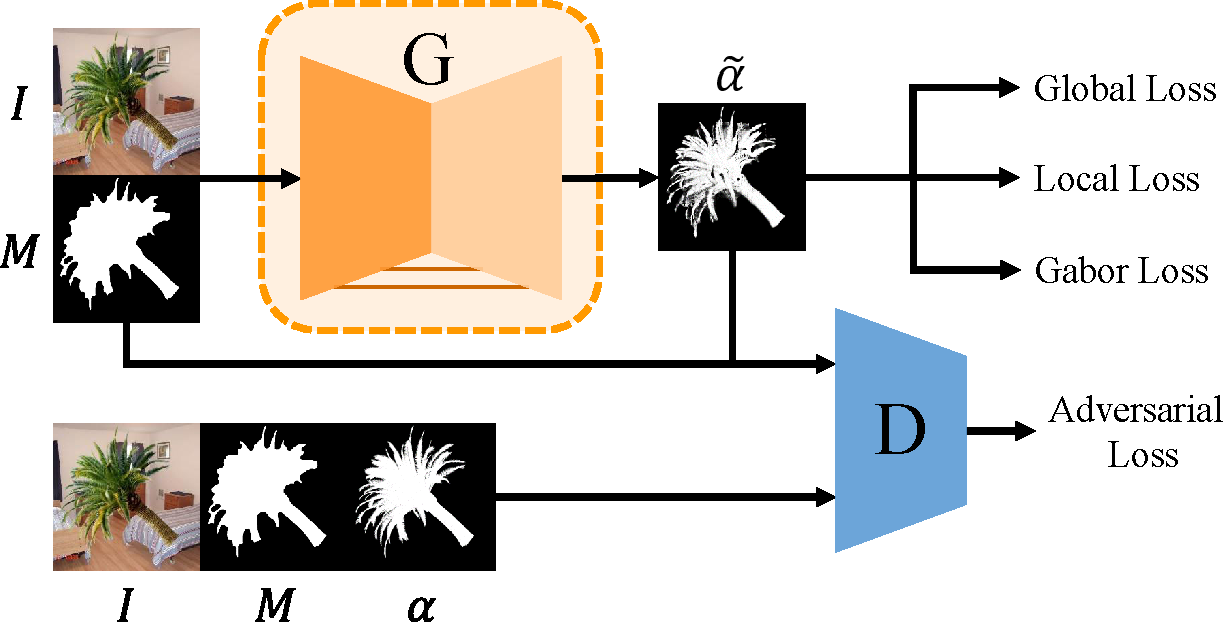
\includegraphics[width = 0.75\columnwidth]{chap6/archtecture.pdf}
	\bicaption{所提出架构示意图}{An illustration of our architecture}
	\label{fig6:archtecture}
\end{figure}
\begin{figure}[t]
	\centering
	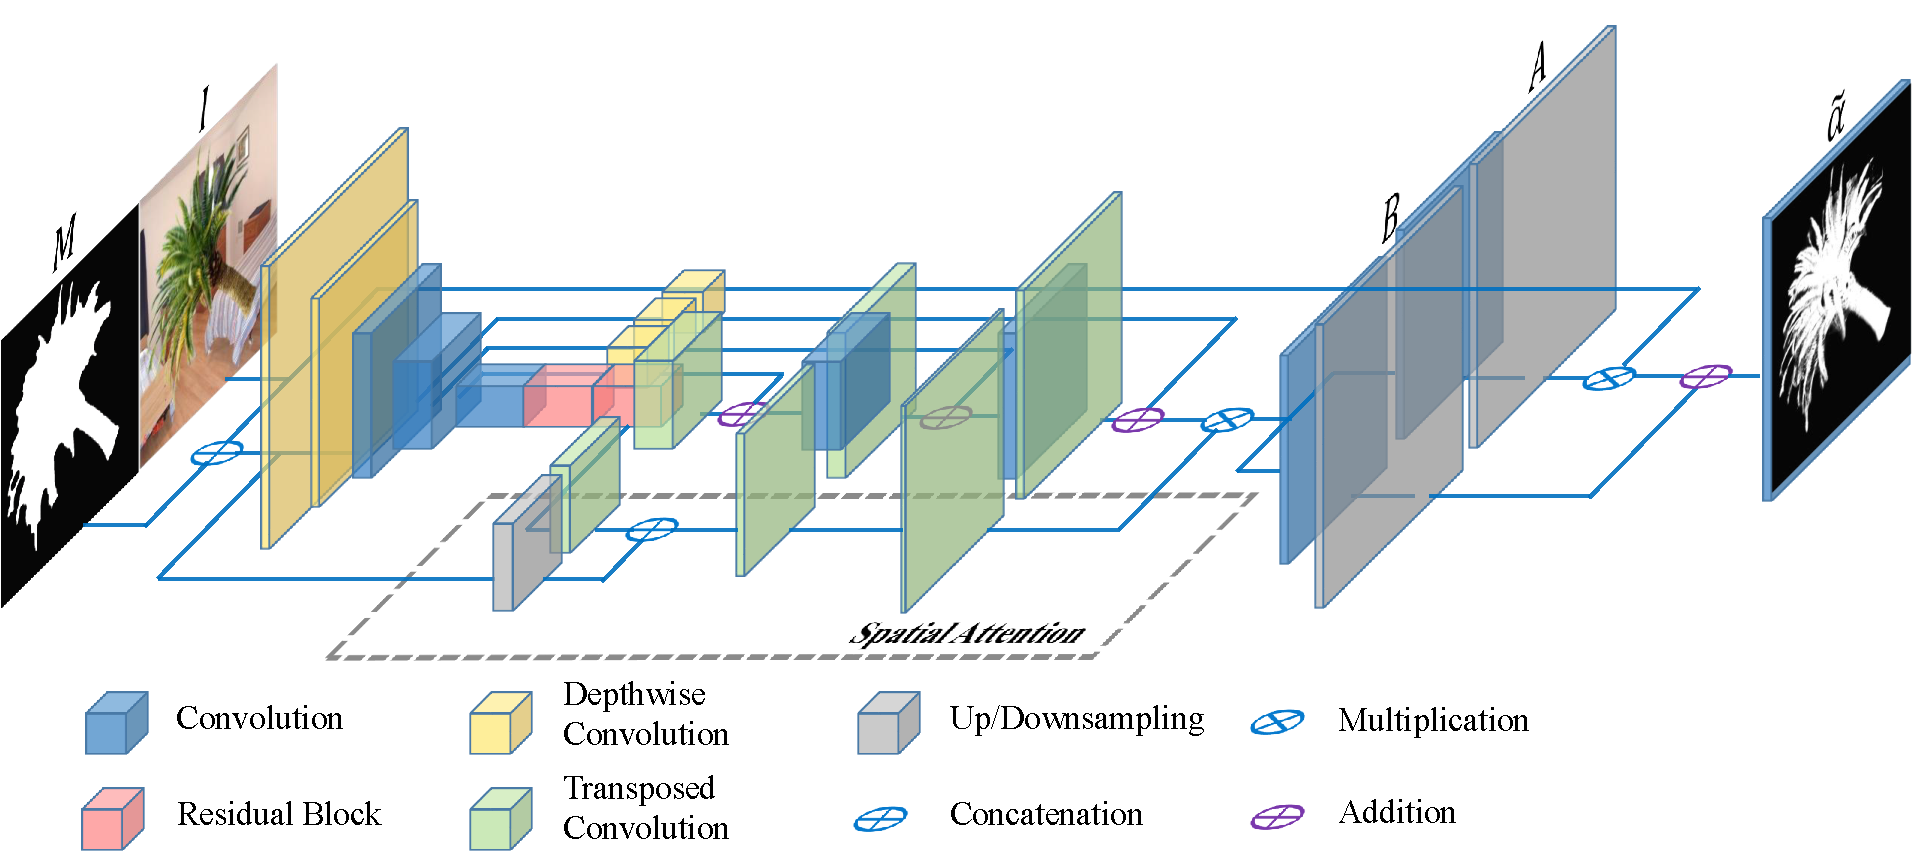
\includegraphics[width = 0.95\columnwidth]{chap6/generator.pdf}
	\bicaption{所提出生成器的概貌。线性系数$A$和$B$从共享相同主干网络的两个分支中生成。最右侧两个缩放系数为4的上采样层用于模仿快速引导滤波器\cite{he2015fast}以加快推理速度}{The overview of our generator. Linear coefficients $A$ and $B$ are generated from two branches sharing the same backbone. The right-most two upsampling layers both have a factor 4 which mimic Fast Guided Filter \cite{he2015fast} for acceleration
	}
	\label{fig6:generator}
\end{figure}

\section{归纳引导滤波器方法}
归纳引导滤波器方法将建立一个高效的、以弱标注分割蒙版为输入的图像抠图网络模型。为此,我们采用了引导滤波器\cite{he2010guided}中的线性模型假设,而引导滤波器正由于其具有的保梯度先验,得以稳定且高效地实现其滤波器功能。
借鉴文献\parencite{lutz2018alphagan}的设计,我们在模型中采用生成对抗网络\cite{goodfellow2014generative}结构。图\ref{fig6:archtecture}中粗略说明了所提出方法的网络架构,图\ref{fig6:generator}中详细介绍了所提出的生成器。

\subsection{归纳引导滤波器的公式化}
\label{sec6:igf}
在引导滤波器\cite{he2010guided}对于图像抠图问题的建模中的基本假设为,输出alpha遮罩图为引导图像$I$在中心点为像素$k$的邻域$\omega_k$内的线性变换:
\begin{equation}
\alpha_i = A_{k}I_{i} + B_{k}, \forall i \in \omega_k,
\end{equation}
其中$ A_{k} $ 和 $ B_{k} $为待优化的线性系数。该线性假设同样被用于Closed-form Matting\cite{levin2008closed}方法中。在弱标注蒙版作为输入的情况下,引导滤波器中的优化目标为在对$A_{k}$进行L2正则化下最小化输出$\alpha_i$与其在弱标注蒙版$ M $上相对应的像素值$M_i$的平方误差。在图像抠图的设定下,引导滤波器对每对输入图像和分割蒙版分别求解优化问题,以获得从输入图像$I$到尽可能相似于蒙版$M$的预测值$\alpha$的线性变换。该线性变换要求了alpha遮罩图需要具有与输入图像近似相同的梯度方向,即$ \nabla \alpha_i=A_k \nabla I_i $。该等式可以被看作为隐含的保梯度先验。

尽管引导滤波器可以作为一种对具有弱标注输入的图像抠图任务的快速且有效的方法,但其受限于最优alpha遮罩与弱标注蒙版之间的差异应充分小这一约束。 从经验上讲,来自语义分割方法或用户交互的分割蒙版与真实标注的alpha遮罩值会有较大的差异。

不同于引导滤波器,本章所提出的方法通过监督学习任务而不是优化问题实现图像抠图。在所提出的方法中,我们仅引入了保梯度先验而舍弃了引导滤波器中的目标函数即alpha预测值与输入蒙版之间的约束。该基于线性变换假设的归纳模型可以有效利用图像抠图数据集中的真实标注信息。我们将所提出的归纳引导滤波器公式化为:
\begin{equation}
\alpha = \phi_{A}(I, M)\circ I + \phi_{B}(I, M), 
\label{eq6:igf}
\end{equation}
式中$ \circ $ 表示哈达玛积(Hadamard product),且我们通过神经网络$ \phi_{A}(I, M) $ 和 $ \phi_{B}(I, M) $ 对引导滤波器中的$ A $ 和 $ B $ 进行参数化。网络 $ \phi_{A} $ 和 $ \phi_{B} $ 以原始图像 $ I $ 及分割蒙版$ M $作为输入,共享网络主干参数(见图\ref{fig6:generator})。归纳引导滤波器方法的优化目标为最小化预测alpha值与真实标注值之间的alpha预测损失。

对于任意的输入图像和分割蒙版,网络$ \phi_{A} $ 和$ \phi_{B} $ 可以生成特定的系数图$ A $ 及 $ B $,以构建出用于生成alpha遮罩估计的线性变换。 
由于 $ \phi_{A} $ 与 $ \phi_{B} $为卷积网络且最后一层为上采样层,从低分辨率特征图中经过上采样得到的$ A $ 和 $ B $,相对较为平滑。因此,线性变换系数图$ A $ 和 $ B $的梯度充分小,可以满足 $ \nabla \alpha \approx A \circ \nabla I $。
由于这一特性,所提出的网络结构可以内在地保持图像本身的梯度方向。

文献\parencite{zhu2017fast}中也提及了相似的思想方法。归纳引导滤波器与其主要区别在于,文献\parencite{zhu2017fast}参考引导滤波器的闭式解公式对其网络中的羽化模块进行定义,该定义丢失了输入图像本身的梯度信息,而仅保留了输入的分割蒙版的边缘和梯度信息。
其羽化模块被定义为:
\begin{equation}
\alpha_i = A_k M^F_i + B_k M^B_i + C_k, \forall i \in \omega_k,
\label{eq6:mobilematitng}
\end{equation}
其中$ M^F $ 和$M^B$ 分别为前景和背景的分割蒙版,$ A_k$、$B_k $和$ C_k $ 为由神经网络生成的系数图。根据公式(\ref{eq6:mobilematitng})可以推导出此羽化模块仅能够保留分割蒙版的梯度方向和边缘,而不是输入图像的梯度。这可以被看作是作用于分割蒙版上的注意力机制。因此,输入的误差较大的分割蒙版可能会造成明显的抠图效果下降。相对应的,归纳引导滤波器可以被看作是输入图像上的注意力机制。这一点与引导滤波器中的线性变换相同,同时也对输入分割蒙版中的噪声更加鲁棒。

\subsection{归纳引导滤波器中的相似性学习}
本节中,我们将从两方面对归纳引导滤波器中数据驱动的相似性学习性质进行讨论。一方面,我们将介绍原始引导滤波器方法中对图像像素间相似性的利用方法,并讨论归纳引导滤波器中数据驱动的学习能力。另一方面,我们将讨论归纳引导滤波器与前文所提出的引导上下文注意力机制的潜在联系。

首先,根据文献\parencite{he2010guided}的推导,引导滤波器的闭式解可以写作约束图的滤波器形式,即:
\begin{equation}
	\alpha_i = \sum_j w_{ij}(I)M_j,
\end{equation}
其中滤波器核$w_{ij}$的权重可以表示为:
\begin{equation}
	w_{ij}(I) = \frac{1}{|\omega|^2} \sum_{(i,j)\in \omega_k}(1+\frac{(I_i-\mu_k)(I_j-\mu_k)}{\sigma^2_k+\epsilon}),
\end{equation}
式中$\mu_k$和$\sigma^2_k$分别表示图$I$在$\omega_k$内的均值和方差。该滤波器形式的闭式解,实现了在局部邻域上根据图像像素间的相似性,对约束图(trimap图或分割蒙版)的信息传播。
同时,根据其讨论,引导滤波器与Closed-form Matting\cite{levin2008closed}中的图拉普拉斯矩阵具有密切的联系。一般性抠图问题的优化问题可写为:
\begin{equation}
	\mathop{\mathrm{min}}\; (\alpha-M)^T\Lambda(\alpha-M)+\alpha^T L\alpha,
	\label{eq6:closed}
\end{equation}
其中$\alpha$为向量化后的alpha遮罩值,$M$为相应的向量化后的约束图,$L$为用于抠图的拉普拉斯矩阵,$\Lambda$为对角权重矩阵。该优化问题可以通过求解线性系统:
\begin{equation}
	(L+\Lambda)\alpha=\Lambda M,
\end{equation}
对于Closed-form Matting方法,该优化问题中的拉普拉斯矩阵定义为:
\begin{equation}
	L_{ij} = \sum_{(i,j)\in \omega_k}(\delta_{ij}-\frac{1}{|\omega|} (1+\frac{(I_i-\mu_k)(I_j-\mu_k)}{\epsilon+\sigma^2_k})),
\end{equation}
式中$\delta_{ij}$为克罗内克$\delta$函数(Kronecker delta)。由此可知,该拉普拉斯矩阵与引导滤波器的滤波器权重间存在等式关系:
\begin{equation}
	L_{ij}=|\omega|(\delta_{ij}-w_{ij}).
\end{equation}
根据文献\parencite{he2010guided},在$\Lambda_{ii}=|\omega|w_{ii}$的情况下,引导滤波器的解可以看做优化问题(\ref{eq6:closed})在一步雅可比迭代(Jacobi iteration)后的近似解。在本章所提出的归纳引导滤波器中,原始引导滤波器中的待优化系数$A$与$B$被参数化为输入图像和分割蒙版的函数,即神经网络$ \phi_{A}(I, M) $ 和 $ \phi_{B}(I, M) $。借助大量的有监督信息的训练数据对神经网络$ \phi_{A}(I, M) $ 及 $ \phi_{B}(I, M) $中的权重参数进行学习,根据由数据归纳学习到的网络,对不同的输入图像及蒙版,生成其特定的引导滤波器系数。区别于原始引导滤波器中仅根据输入本身生成滤波器算子权重的方式,归纳引导滤波器可以利用在监督数据中学习得出的一般性规则生成相应滤波器。

另一方面,通过将图\ref{fig6:generator}神经网络的最后一层卷积计算及其前一层的空间注意力机制引入公式(\ref{eq6:igf})中可以近似得到前文所提出的局部的引导上下文注意力机制的传播效果。
此处,首先假设$ \phi_{A}(I, M) $的输出特征及图像$I$为单通道以保持公式简洁,令$w^A\in \mathbb{R}^{m\times n\times l}$、$w^B\in \mathbb{R}^{m\times n\times l}$分别表示网络$ \phi_{A}(I, M) $与$ \phi_{B}(I, M) $最后一层卷积操作的卷积核,$\omega$表示卷积核的空间位置下标集合,将输入特征通道以向量形式表示则有:
\begin{equation}
	\begin{aligned}
	&\phi_{A}(I, M)_{ij} = \sum_{m,n\in \omega} (w^A_{mn})^T(f_{i+m,j+n}\circ g_{i+m,j+n}), \\&\phi_{B}(I, M)_{ij} = \sum_{m,n\in \omega} (w^B_{mn})^T(f_{i+m,j+n}\circ g_{i+m,j+n}),
	\end{aligned}
\end{equation}
其中$f$为输入图像$I$与弱标注分割蒙版$M$通过主干网络生成的深层alpha遮罩特征,$g$表示由分支网络生成的包含有低级图像信息的注意力图,此处省略$(I,M)$以保持公式简洁。将其带入公式(\ref{eq6:igf})中可得:
\begin{equation}
	\begin{aligned}
	\alpha_{ij} =& \sum_{m,n\in \omega} (I_{ij}w^A_{mn}+w^B_{mn})^T(f_{i+m,j+n}\circ g_{i+m,j+n})\\
	=& \sum_{m,n\in \omega} (I_{ij}w^A_{mn})^T(g_{i+m,j+n}\circ f_{i+m,j+n}) + \sum_{m,n\in \omega} (w^B_{mn})^T(f_{i+m,j+n}\circ g_{i+m,j+n})\\
	=& \sum_{m,n\in \omega} (w^A_{mn}\circ g_{i+m,j+n}I_{ij})^Tf_{i+m,j+n} + \sum_{m,n\in \omega} (w^B_{mn})^T(f_{i+m,j+n}\circ g_{i+m,j+n})
	\end{aligned}
	\label{eq6:localhop}
\end{equation}
则公式(\ref{eq6:localhop})中等式右侧第一项可以认为是具有低级图像信息的特征$w^A_{mn}\circ g_{i+m,j+n}$中每个空间位置及输入通道分别与图像$I$中$(i,j)$位置的信息计算相似度后,根据相似度对特征$f$进行局部的聚合,实现信息传播效果,其中的$w^A$也可以视为根据位置编码对相似度进行加权的可学习参数。而第二项可以看作对注意力激励后的特征$f\circ g$进行的常规卷积计算操作以起到残差效果。由于卷积核$w^A$及包含低级图像特征的$g$具有可学习性,所以此结构可以近似局部HOP模块的效果。

\subsection{生成器设计}
本节所提出的生成器结构包括了一个轻量级的类Hourglass\cite{newell2016stacked}主干,一个空间注意力机制及一个线性变换。鉴于U-Net\cite{ronneberger2015u} 及Hourglass \cite{newell2016stacked}网络结构被证明可以有效地从高分辨率的网络特征中保留低级图像信息,本生成器的网络主干参考了以上两种结构。同时由于深度可分离卷积(depthwise separable convolution)在轻量级深度神经网络中被广泛采用\cite{chollet2017xception,howard2017mobilenets,zhang2018shufflenet,sandler2018mobilenetv2},我们使用深度可分离模块构造网络的前两层卷积操作以及跳层连接中的计算模块。需要注意的是,生成器在结构设计上参考了文献\parencite{nekrasov2018real},仅在具有高分辨率特征映射的卷积层上引入深度可分离卷积操作。上述设计细节的核心动机都集中于降低网络在预测阶段的计算时延。除此之外,由于采用了梯度先验,该生成器网络可以模仿快速引导滤波器\cite{he2015fast}的设计方式,只输出alpha遮罩尺寸四分之一的特征映射,并通过四倍上采样进行最后的线性变换。这一步操作直接地避免了在高分辨率特征上进行密集的运算,可以降低近一半地预测时延。

部分先前的深度图像抠图方法\cite{chen2018semantic,zhu2017fast}在其网络结构中采用了空间注意力机制\cite{xu2015show},并得到了显著优异的抠图效果。对于本节所提出的生成器结构中的注意力机制,我们通过对输入图像及编码器输出特征进行信息融合,计算出同时具有低级图像信息及高级语义信息的注意力图,并将其作用于解码器中的高分辨特征上。

除了判别器所需要的对抗损失之外,我们在生成器的输出上增加了三个损失进行监督:全局损失、局部损失和Gabor损失。下文中分别用$ \hat{\alpha} $ 和 $ {\alpha} $表示alpha遮罩预测值和标注值。

\begin{itemize}
	\item \textbf{全局损失}。为对alpha遮罩预测值进行整体的监督,通过alpha真值与估计值之间的平均L1损失构造的全局损失被加入到损失函数中用于模型训练:
	\begin{equation}
	\mathcal{L}_g = \frac{1}{|\alpha|}\|\alpha-\hat{\alpha}\|_1, 
	\end{equation}

	\item \textbf{局部损失}。当我们在对抠图网络进行训练时,除全局损失之外,我们希望目标函数更加集中在前景物体的边缘部分。局部损失是一个基于误差指示函数$ \Delta(\alpha, M) = \delta(|\alpha - M|>\epsilon) $定义的加权重构损失。该误差指示函数输出一个二值边缘图,其中在alpha标注值和输入的分割蒙版具有不同值的位置为$1$,其他位置为$0$。$ \delta $函数使得低于$ \epsilon $误差值在该误差指示函数中被忽略。在损失函数中,我们采用$ \epsilon=0.01 $。则局部损失函数可以被定义为: 
	\begin{equation}
	\mathcal{L}_l = \frac{1}{\sum \Delta(\alpha, M)}\|\Delta(\alpha, M) \circ (\alpha-\hat{\alpha})\|_1.
	\end{equation}
	在实际实现中,我们对误差指示函数输出的二值边缘图用$ 7\times 7 $的核进行形态学膨胀,以获得更大的边缘区域。

	\item \textbf{Gabor损失}。感知损失(perceptual loss)\cite{johnson2016perceptual}被证明可以在图像转换任务中显著地改进预测图的视觉质量。感知损失使用了VGG网络\cite{simonyan2014very}在具有特定类别的RGB图像上进行分类训练的预训模型构造损失,可以同时评估预测图与真值图之间的纹理及语义区别。而在通用图像抠图任务上,感知损失中的语义部分相对属于冗余信息,而单通道alpha遮罩的数据分布也区别于RGB图像。因此,我们在图像抠图任务中提出了与感知损失具有相似性的Gabor损失。Gabor损失将感知损失中预训练的多层卷积核替换为单层的Gabor滤波器集合,以提取高频特征。由于Gabor滤波器与神经网络中浅层学习到的卷积核具有一定的相似性,一些先前的工作\cite{ouyang2013joint}将Gabor滤波器作为卷积核或卷积核的初始化引入神经网络中。因此,我们将Gabor损失定义为:
	\begin{equation}
	\mathcal{L}_{gb} = \frac{1}{|\alpha||\Phi|}\sum_{\phi_{gb}\in \Phi}\|\phi_{gb}(\alpha)-\phi_{gb}(\hat{\alpha})\|_2^2,
	\end{equation}
	其中函数$ \phi_{gb}(\cdot)$ 表示采用Gabor滤波器进行的卷积计算,$ \Phi $为不同的Gabor滤波器集合。在训练中,我们在集合$ \Phi $内设计了16个不同方向的$5\times5$ Gabor滤波器。所有的滤波器均有波长$\lambda=5$,空间纵横比(spatial aspect ratio)$\gamma=0.5$,标准差$\sigma=0.5$。我们在实验中尝试了使用不同的波长及标准差构造更大的滤波器集合,并不会对最终效果产生显著的提升。一些深度抠图方法基于相同的动机在目标函数中引入了梯度损失\cite{levinshtein2018real,chen2019boundary,samplenet}。相对于梯度,Gabor损失可以被看作是梯度损失基础上的扩展版本,可以提取更加全面的高频特征。
\end{itemize}


\begin{figure}[t]
	\centering
	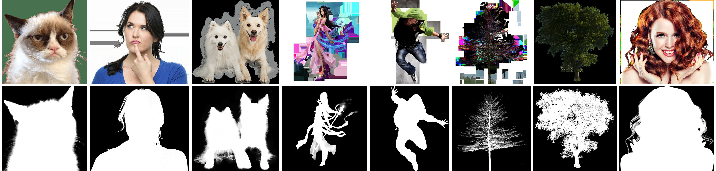
\includegraphics[width = 1\columnwidth]{chap6/dataset_foreground.pdf}
	\bicaption{MAT-2793数据集中部分前景物体样例}{Some foreground object samples from the MAT-2793 dataset}
	\label{fig6:foreground}
\end{figure}

\begin{figure}[t]
	\centering
	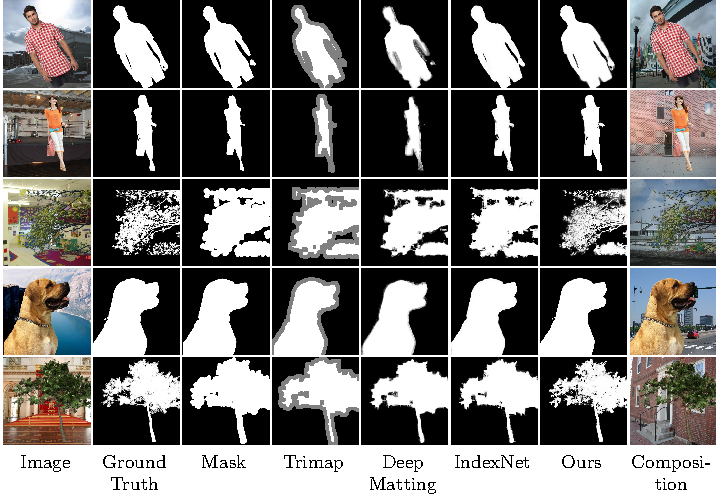
\includegraphics[width = 1\columnwidth]{chap6/test_versa.pdf}
	\bicaption{MAT-2793数据测试集上的视觉对比结果。Trimap图仅用于Deep Matting及IndexNet方法。合成图由所提出方法预测结果与随机背景合成}{The visual comparison results on MAT-2793 testing set. The trimap is only for Deep Matting and IndexNet. The composition is composed with our results and random backgrounds}
	\label{fig6:test-data}
\end{figure}

\subsection{判别器设计}
在AlphaGAN\cite{lutz2018alphagan}的生成对抗结构中,算法首先通过生成器预测出的alpha遮罩合成新的合成图像,然后将原始trimap图以及新的合成图像作为判别器输入。由于图像抠图任务几乎不关注语义信息,所以该设计在判断一张合成图是否真实这一点上的定义是模糊的。即使通过一个不完整的或者不正确alpha遮罩图合成图像,也可以认为是一张正常合成的图像,同时可以具有很高的保真度。因此将由真实alpha遮罩合成的图像作为正样本而将由网络预测的alpha遮罩合成的图像作为负样本,本身具有极大的判别难度。为解决这个问题,我们将条件三元组作为判别器的输入,包括原始图像、弱标注分割蒙版及alpha遮罩图。这一设计类似于一些采用图像对作为判别器输入的图像生成方法\cite{hu2018pose}。给定一个三元组输入,判别器可以对输入的自洽性(self-consistency)进行判别。具体来说,判别器被设计为在给定原输入图像和分割蒙版的条件下,判断一个预测出的alpha遮罩图是否正确,而不是单纯判断alpha遮罩或其合成图像是否真实。

\begin{itemize}
	\item \textbf{对抗损失}。在判别器方面,我们采用LSGAN\cite{mao2017least}及梯度惩罚\cite{gulrajani2017improved}作为对抗损失。损失函数定义为:
	\begin{equation}
	\begin{aligned}
	\mathcal{L}_{adv} =\; & \mathcal{L}_D + \mathcal{L}_G + \lambda_{gp}  \mathbb{E}_{\tilde{\alpha}}[(\|\nabla_{\tilde{\alpha}}D(\tilde{\alpha}|I, M)\|_2-1)^2]\\
	\mathcal{L}_D =\; & \mathbb{E}_\alpha[(D(\alpha|I, M)-1)^2] + \mathbb{E}_{\hat{\alpha}}[D(\hat{\alpha}|I, M)^2]\\
	\mathcal{L}_G =\; & \mathbb{E}_{\hat{\alpha}}[(D(\hat{\alpha}|I, M)-1)^2],
	\end{aligned}
	\end{equation}
	其中,$ \tilde{\alpha} $为$ \alpha $ 与 $ \hat{\alpha} $的凸组合,组合系数随机采样于均匀分布,同时我们采用超参数$ \lambda_{gp} =10 $。
\end{itemize}

\begin{table}[t]
	\setlength{\tabcolsep}{16pt}
	\bicaption{在MAT-2793数据测试集上的数值结果}{The quantitative results on the MAT-2793 testing set}
	\centering
	\begin{tabular}{lcccc}  
		\toprule
		Methods & MSE & SAD & Grad  &Conn\\
		\midrule
		Fast Guided Filter\cite{he2015fast}  & 0.101 & 9.57 & 15.53 & 5.53\\
		Adobe DIM\cite{xu2017deep}  & 0.148 & 8.54 & 16.53 & 4.42\\
		Context-aware Matting\cite{hou2019context}  & 0.079 & 5.24  &  12.67 & 2.12 \\
		IndexNet Matting\cite{lu2019indices}  & 0.036 & 3.01 & \textbf{5.86} & 1.75\\
		Ours & \textbf{0.028} & \textbf{2.51} & {6.45} & \textbf{1.51}\\      	
		\bottomrule
	\end{tabular}
	\label{tab6:ours}
\end{table}

本章所提出的归纳引导滤波器的完整损失函数为:
\begin{equation}
\mathcal{L} = \lambda_g \mathcal{L}_g + \lambda_l \mathcal{L}_l + \lambda_{gb} \mathcal{L}_{gb} + \lambda_{adv} \mathcal{L}_{adv},
\end{equation}
其中,我们选择超参数$ \lambda_g = 10$、$\lambda_l = 1$、$\lambda_{gb} = 200 $ 及$ \lambda_{adv} = 1$。

对于判别器部分,我们在实现中引入了能够对生成图像数据中每个区块分别判定保真度的PatchGAN结构\cite{isola2017image},以保证所采用的判别器能够充分地注意到生成alpha遮罩图的局部纹理细节。谱归一化\cite{miyato2018spectral}被证明在生成的对抗网络的训练中可以显著有效地增加训练稳定性,因此,我们在判别器中引入了谱归一化约束。

\begin{figure}[t]
	\centering
	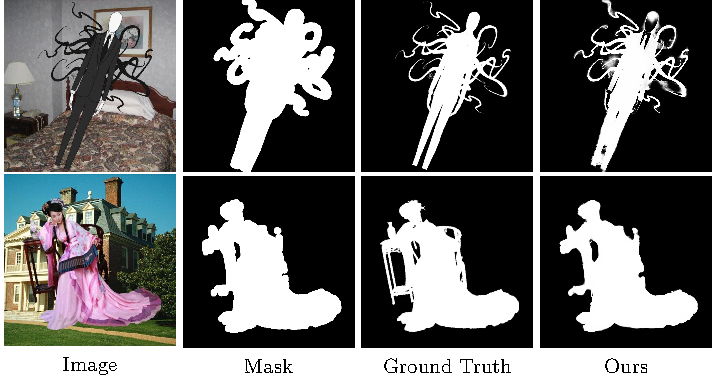
\includegraphics[width = 1\columnwidth]{chap6/fail_versa.pdf}
	\bicaption{MAT-2793数据测试集上的两个失败样例}{Two failed cases on MAT-2793 testing set}
	\label{fig6:failed}
\end{figure}

\section{实验结果}
\begin{figure}[t]
	\centering
	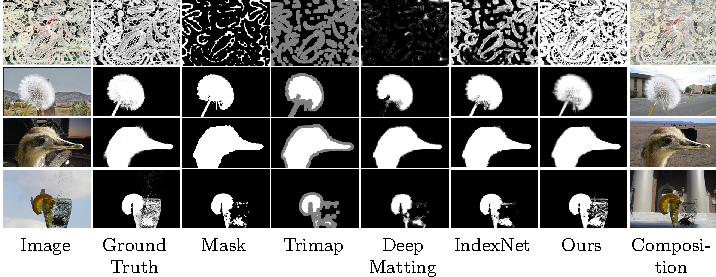
\includegraphics[width = 1\columnwidth]{chap6/test_adobe.pdf}
	\bicaption{在Composition-1k测试集上视觉对比结果。合成图由所提出方法预测结果与随机背景合成}{The visual comparison  on Composition-1k testing set. The composition is composed with our results and random backgrounds}
	\label{fig6:adobe}
\end{figure}
在本节中,我们分别在MAT-2793和Composition-1k\cite{xu2017deep}两个数据集上对所提出的方法进行评估。为验证所提出方法每一部分的有效性,本节进行了大量的消融实验对归纳引导滤波器的每一部分进行了测试,同时我们对所提出方法进行了效率测试并与部分为特定场景设计的实时深度抠图方法进行了效率对比。本节最后我们给出了所提出方法在部分非合成的自然图像上的抠图效果。
\subsection{MAT-2793数据集}
\label{sec6:data}
由于alpha遮罩图标注的难度极大,数据驱动的图像抠图方法一个首要的困境在于训练数据的匮乏。目前已公开的最大的图像抠图训练数据集\cite{xu2017deep}仅包含493张不同的前景物体图。因此,为实现对于弱标注图像抠图任务的训练,我们构造了一个具有2,793张前景物体图像的数据集MAT-2793。数据集中的前景图像及相应的alpha遮罩图采集自互联网,并经过人工筛选,部分前景物体为绘制图像而非自然图像。在图\ref{fig6:foreground}中展示了数据集中部分前景物体图像的样例。我们将数据集划分为具有2,504张前景图的训练集和具有289张前景图的测试集。
在实验中,我们在数据集SUN\cite{xiao2010sun}及ADE20K\cite{zhou2017scene}中选择了约5,000张高分辨率图像作为合成图像的背景。

在训练数据生成及增广方面,我们首先对每个前景物体进行水平翻转并进行11个不同角度的旋转,以生成22个不同的前景图,然后对每张前景图随机选择背景图像进行合成。为生成弱标注的分割蒙版,我们首先将真实的alpha这遮罩图上大于$0.5$的alpha值认为是前景,得到一个初始分割蒙版。然后我们在区间$5\times5$ 到 $30\times30$之间随机采样两个核的尺寸,采用该随机核同时对分割蒙版进行形态学的膨胀与腐蚀。如果生成的分割蒙版中前景部分的区域面积比例不足alpha遮罩中前景部分面积的一半,则该训练样本被抛弃。我们将合成图、相应的alpha遮罩图以及分割蒙版图的短边都缩放至600像素。为进一步增广训练数据,我们对训练图像进行随即剪裁,并将剪裁结果缩放至$512\times512$。同时,在训练阶段我们在区间$ [-40, 40] $内对图像的色度进行随机扰动。由于我们认为在泛化度较高的图像抠图问题中图像的前景及背景具有一定的可交换性,即我们可以在训练阶段对前景及背景的标注进行互换。因此,我们依概率$0.5$对输入分割蒙版的标签进行了随机反转,并采用$1-\alpha$作为真实标注值。在测试阶段,我们采用尺寸为$600\times600$的中心剪裁并将剪裁结果缩放到$512\times512$。

\begin{table}[t]
	\setlength{\tabcolsep}{16pt}
	\bicaption{在Composition-1k测试集上采用弱标注输入的定量测试结果}{The quantitative results on the Composition-1k testing set with weakly annotations}
	%    \small
	\centering
	%     \begin{tabular}{lp{3em}<{\centering}p{3em}<{\centering}p{6em}<{\centering}p{6em}<{\centering}}  
	\begin{tabular}{lcccc}  
		\toprule
		Methods & MSE & SAD & Grad &Conn\\
		\midrule
		Fast Guided Filter \cite{he2015fast} &  0.130 & 176.2  & 150.5  & 111.2 \\
		Deep Matting \cite{xu2017deep} & 0.243 & 105.2 & 55.0 & 56.1\\
		Context-aware Matting \cite{hou2019context}  & 0.103  & 63.0  & 46.6  & 44.4 \\
		IndexNet Matting \cite{lu2019indices}  & 0.084 & 52.2 & \textbf{33.2} & \textbf{33.8}\\
		Ours & \textbf{0.064} & \textbf{46.2} & {42.1} & {35.7}\\        
		\bottomrule
	\end{tabular}
	\label{tab6:adobe}
\end{table}

\subsection{MAT-2793测试集实验结果}
为在不同的抠图方法之间进行公平的对比\footnote{在本节的对照实验中采用了第三方实现的项目https://github.com/foamliu/Deep-Image-Matting作为未开源的Deep Matting方法的实现。},我们根据训练数据中每张合成图的分割蒙版生成对应的trimap图作为部分需要trimap的抠图方法的输入数据。为在分割蒙版上构造trimap图所需要的不确定区域,我们选用尺寸为$20\times20$分别对分割蒙版图进行形态学膨胀和腐蚀,以生成不确定区域。最终的评估误差仅在不确定区域中计算。需要注意的是,由于分割蒙版本身具有明显的噪声,因此在自动生成的trimap图中也存在一定的标注错误现象。
在本节的实验中,我们对快速引导滤波器\cite{he2015fast}进行了实现,并选取降采样系数为4。在实验效果的评价指标方面遵循了文献\parencite{rhemann2009perceptually}的建议,采用了均方误差(Mean Square Error,MSE)、总绝对差(Sum of Absolute Difference,SAD)、梯度误差(Gradient error,Grad)和连通误差(Connectivity error,Conn)四个评估测度。表\ref{tab6:ours}展示了不同抠图算法在MAT-2793测试数据集上的定量评估结果。此外,我们在图\ref{fig6:test-data}中对不同算法在测试集上的估计结果进行了视觉效果的对比。结果表明,我们所提出的方法对输入的分割蒙版中的噪声具有一定的鲁棒性,同时相比于其他目前最先进的图像抠图方法具有一定的竞争力。


在图\ref{fig6:failed}中,我们展示了两个典型的alpha遮罩预测失败样例。预测失败的原因分为两种主要情况,其一为图\ref{fig6:failed}中第一行所示的抠图算法由于缺少明确的前、背景指示信息而导致对前景和背景信息产生混淆,而将前景物体的一部分作为背景进行预测,或将背景中显著部分作为前景。其二为图\ref{fig6:failed}第二行中所示的,由于前景与背景结构复杂且所输入的分割蒙版在部分重要区域中与alpha遮罩信息差距过大,从而使得网络无法正确识别到前景物体,导致alpha遮罩预测图的整体性退化。

\subsection{Composition-1k测试集实验结果}
Composition-1k测试集\cite{xu2017deep}包含有50个不同的前景图生成的1,000张合成测试图。在实验中,我们采用与MAT-2793测试数据集完全相同的方式生成测试数据对应的弱标注分割蒙版。在根据弱标注分割蒙版生成trimap图阶段,考虑到Composition-1k测试集中侧视图尺寸较大的问题,我们在腐蚀与膨胀操作中选取了尺寸为$50\times50$的核。trimap图生成结束后,所有数据图片被缩放至$512\times512$用于alpha遮罩预测。最后,预测结果被缩放回原图大小,然后在生成的trimap图中的不确定区域内进行误差计算。我们在图\ref{fig6:adobe}中对不同算法在Composition-1k测试集上的预测结果进行了视觉效果上的对比,同时在表\ref{tab6:adobe}中对预测alpha遮罩在不同损失测度下的定量评估结果进行了数值比较。在Composition-1k测试集上的实验结果同样表明了,本章所提出的方法具有处理弱标注输入的能力。

\begin{table}[t]
	%	\small
	\setlength{\tabcolsep}{8pt}
	\centering
	\bicaption{在MAT-2793数据测试集上消融实验的定量结果}{The quantitative results of ablation study on the MAT-2793 testing set}
	%     \begin{tabular}{lp{3em}<{\centering}p{3em}<{\centering}p{6em}<{\centering}p{6em}<{\centering}} 
	\begin{tabular}{lcccc}
		\toprule
		Methods & MSE & SAD & Grad &Conn\\
		\midrule
		Ours & \textbf{0.028} & \textbf{2.51} & \textbf{6.45} & \textbf{1.51}\\    
		w/o Atten & 0.037 & 2.95& 8.65 & 1.70\\
		w/o Gabor & 0.031 & 2.68 & 7.15 & 1.55\\
		w/o IGF & 0.034 & 2.81 & 8.3 & 1.62\\
		w/o Adv & 0.042 & 3.33 & 9.1 & 1.87\\
		w/o IGF w/ FB  & 0.034 & 2.84 & 8.35 & 1.65\\
		w/o Gabor w/ Grad & 0.030 & 2.68 & 6.96 & 1.57\\
		w/o Gabor w/ Percep & 0.029 & 2.67 & 6.77 & 1.61\\
		\bottomrule
	\end{tabular}
	\label{tab6:ablation}
\end{table}
\subsection{消融实验}
在本节中,我们通过移除模型中的不同部分然后对所提出模型进行评估,以展示空间注意力机制(Atten)、Gabor损失(Gabor)、对抗损失(Adv)及梯度先验(IGF)各自的有效性。在所提出的方法中移除梯度先验表示我们对网络生成的系数图$A$与$B$拼接后进行逐点卷积(point-wise convolution)以获取最终的alpha遮罩预测,而不计算系数$A$与输入图像的乘积。在这种情况下,生成器部分可以被看成是一个通用的自编码器。表\ref{tab6:ablation}报告了消融实验的定量评测结果。此处值得注意的一点在于,尽管空间注意力机制部分对最终预测效果有显著的贡献,但同时也向神经网络中引入了更多的运算量。
由于本章所提出的梯度先验与文献\parencite{zhu2017fast}中的所提出的羽化模块(FB)具有一定的相似性,故此我们将公式(\ref{eq6:igf})中的梯度先验替换为公式(\ref{eq6:mobilematitng})中的羽化模块,并在表\ref{tab6:ablation}对其效果进行了对比,将梯度先验替换为羽化模块的模型以\textit{w/o IGF w/ FB}表示。

此外,在表\ref{tab6:ablation}中我们同样将训练中的Gabor损失替换为梯度损失(Grad)或感知损失(Percep)进行效果对比,以显示Gabor损失在该问题中的有效性。

\begin{table}[t]
	\setlength{\tabcolsep}{8pt}
	\bicaption{在CPU及移动设备上的速度评估结果}{The results of speed evaluation on CPU and mobile devices}
	\centering
	%	\begin{savenotes}
	\begin{tabular}{lccc}  
		\toprule
		Methods  & Input Size&  Device & Time (ms)   \\
		\midrule\midrule
		HairMatteNet\cite{levinshtein2018real}& 224x224& iPad Pro GPU & 30   \\
		\midrule
		\multirow{2}{*}{LDN+FB\cite{zhu2017fast}} &\multirow{2}{*}{128x128}  &  Core E5-2660 & 38  \\
		&&  Adreno 530 & 62  \\
		\midrule
		\midrule
		Fast Guided Filter\cite{he2015fast} &512x512 & Core i5-9400 & 81.1  \\
%		 & Core i7-7700& 62.0  \\
		\midrule
		Deep Matting\cite{xu2017deep}& 512x512& Core i5-9400 & 942.6  \\
%		  & Core i7-7700 & 4003.2  \\
		\midrule
		IndexNet Matting\cite{lu2019indices} &512x512	& Core i5-9400 & 604.2  \\
		\midrule
		Context-aware Matting\cite{hou2019context}& 512x512	& Core i5-9400 & 7805.3  \\
		\midrule
		\multirow{3}{*}{Ours} &\multirow{3}{*}{512x512}& Core i5-9400 & 13.2  \\
		&& iPhone Xs   & 15.7  \\
%		& iPhone X    & 22.3   \\
		&& iPhone SE  & 25.9   \\
%		& Core i7-7700 & 13.0  \\
		\bottomrule
	\end{tabular}
	\label{tab6:time_mobie}
\end{table}

\subsection{效率评估实验结果}
为验证所提出的抠图模型的推理效率,我们包括CPU及移动设备在内等不同平台上分别对所提出方法进行速度测试和对比。部分在文献中提供了效率测试实验的用于人像(LDN+FB \cite{zhu2017fast})或头发(HairMatteNet \cite{levinshtein2018real})的实时抠图算法也同时被加入对比。我们在实验结果中报告了这些算法在原始文献中提供的效率实验的测试数据。在表\ref{tab6:time_mobie}中,我们展示了不同方法在CPU及不同的移动设备上的速度评估结果。我们通过Apple CoreML框架将所提出的模型部署在不同型号的iPhone设备上。可以注意到,在接受$512\times512$的图像作为输入数据的情况下,所提出的方法依然可以在2016年出产的iPhone SE设备上达到实时运算的效果。此外,我们在Nvidia的GPU设备上对不同方法的运行效率进行了评估

\begin{table}[h]
	\bicaption{在Nvidia GPU设备上的速度评估结果。我们对所提出的方法同时展示了考虑及不考虑GPU I/O情况下的速度结果}{The results of speed evaluation on Nvidia GPU devices. We also display the speed of our method with or without GPU I/O}
	\centering
	\begin{tabular}{lcccc}  
		\toprule
		Methods & Input Size& Device & BatchSize & Time (ms)\\
		\midrule
		\midrule
		BANet-64\cite{chen2019boundary}& 512x512  & 1080 Ti& 1  & 23.3 \\
		\midrule
		LDN+FB\cite{zhu2017fast} &128x128 & TITAN X & 1& 13  \\
		\midrule
		\midrule
		Deep Matting\cite{xu2017deep}& 512x512  &  1080 & 1  & 81.8 \\
		\midrule
		IndexNet Matting\cite{lu2019indices} &512x512  &  1080 & 1  & 38.4 \\
		\midrule
		Context-aware Matting\cite{hou2019context}& 512x512  &  1080 & 1  & 710.7 \\
		\midrule
%		\multirow{2}{*}{Ours w/ I/O (512x512)} & \multirow{2}{*}{ V100} &  1  & 3.48 \\
%		&&   256 & 1.46  \\
%		\midrule
%		\multirow{2}{*}{Ours w/o I/O (512x512)} & \multirow{2}{*}{ V100}  &  1 &  2.19  \\
%		& & 256  & 0.18 \\
%		\midrule
%		\multirow{2}{*}{Ours w/ I/O (512x512)} & \multirow{2}{*}{ 1080Ti} &  1  & 4.20 \\
%		&&   256 & 1.64  \\
%		\midrule
%		\multirow{2}{*}{Ours w/o I/O (512x512)} & \multirow{2}{*}{ V100}  &  1 &  2.19  \\
%		& & 256  & 0.18 \\
%		\midrule
		\multirow{2}{*}{Ours w/ I/O}& \multirow{2}{*}{512x512} & \multirow{2}{*}{ 1080} &  1  & 3.88 \\
		&&&   256 & 1.68  \\
		\midrule
		\multirow{2}{*}{Ours w/o I/O}& \multirow{2}{*}{512x512} & \multirow{2}{*}{ 1080}  &  1 &  2.55  \\
		& && 256  & 0.54 \\
		\bottomrule
	\end{tabular}
	\label{tab6:time_gpu}
\end{table}
\subsection{自然图像抠图效果}
为进一步评估所提出方法在真实自然图像上的表现,我们采用了DeepLab v3+\cite{chen2018encoder}模型作为分割方法,以显示所提出抠图方法在实际应用场景中的表现。在该实验中,我们仅对包含有DeepLab v3+可分割的语义物体的图像进行测试,同时将分割结果直接作为所提出模型的弱标注分割蒙版输入到网络中。
我们首先在PASCAL VOC 2012\cite{everingham2015pascal}语义分割数据的测试集中的部分图像上进行了测试,相应的DeepLab v3+方法分割结果及归纳引导滤波器的抠图结果展示在图\ref{fig6:voc_deeplab}中。同时,部分通过互联网收集的盆栽植物图像以及Supervisely人像分割数据集\cite{Supervise.ly}中图像的抠图结果被展示在图\ref{fig6:plant_sup_deeplab}中。此外,图\ref{fig6:adobe_deeplab}还提供了Composition-1k 测试集\cite{xu2017deep}中部分具有可分割语义物体的图像样本的抠图结果。
\begin{figure}[h]
	\centering
	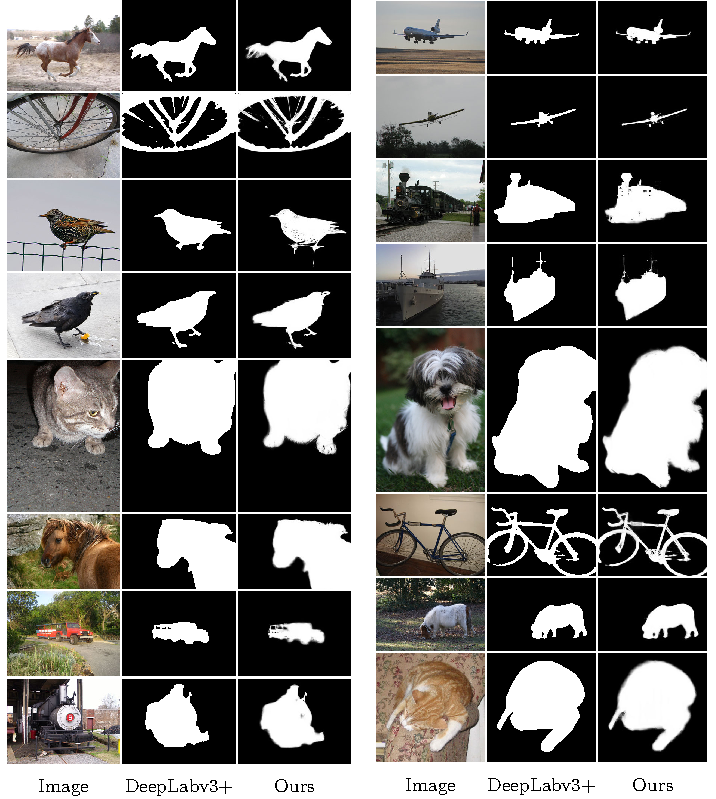
\includegraphics[width = 1\columnwidth]{chap6/voc_deeplab.pdf}
	\bicaption{PASCAL VOC 2012测试集中部分图像抠图结果,分割蒙版由DeepLab v3+生成}{Results of some images in PASCAL VOC 2012 testing set. Masks are generated by DeepLab v3+}
	\label{fig6:voc_deeplab}
\end{figure}
\begin{figure}[h]
	\centering
	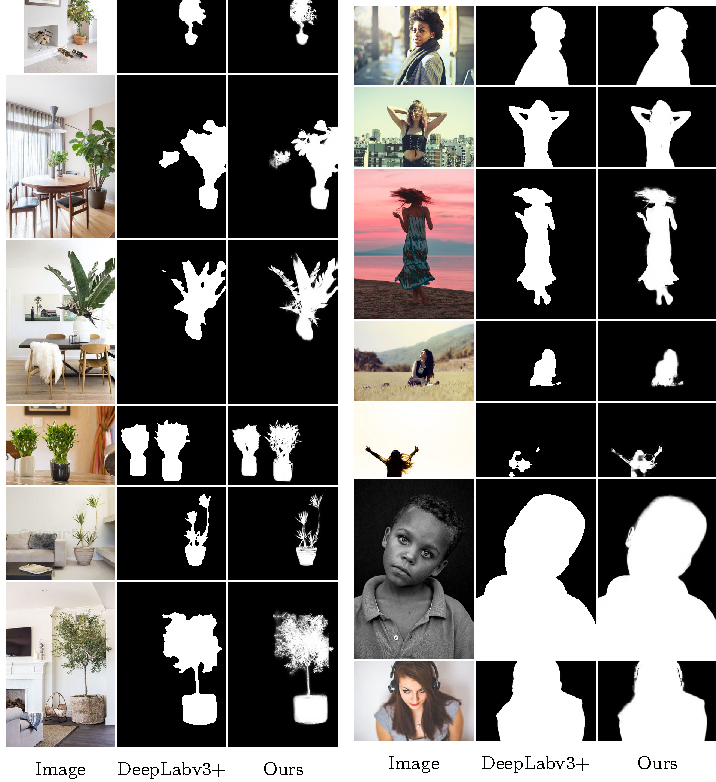
\includegraphics[width = 1\columnwidth]{chap6/plant_sup_deeplab.pdf}
	\bicaption{部分盆栽植物以及Supervisely人像数据集中样本的抠图结果,分割蒙版由DeepLab v3+生成}{Results of some potted plant images and samples from Supervisely Person dataset. Masks are generated by DeepLab v3+}
	\label{fig6:plant_sup_deeplab}
\end{figure}
\begin{figure}[h]
	\centering
	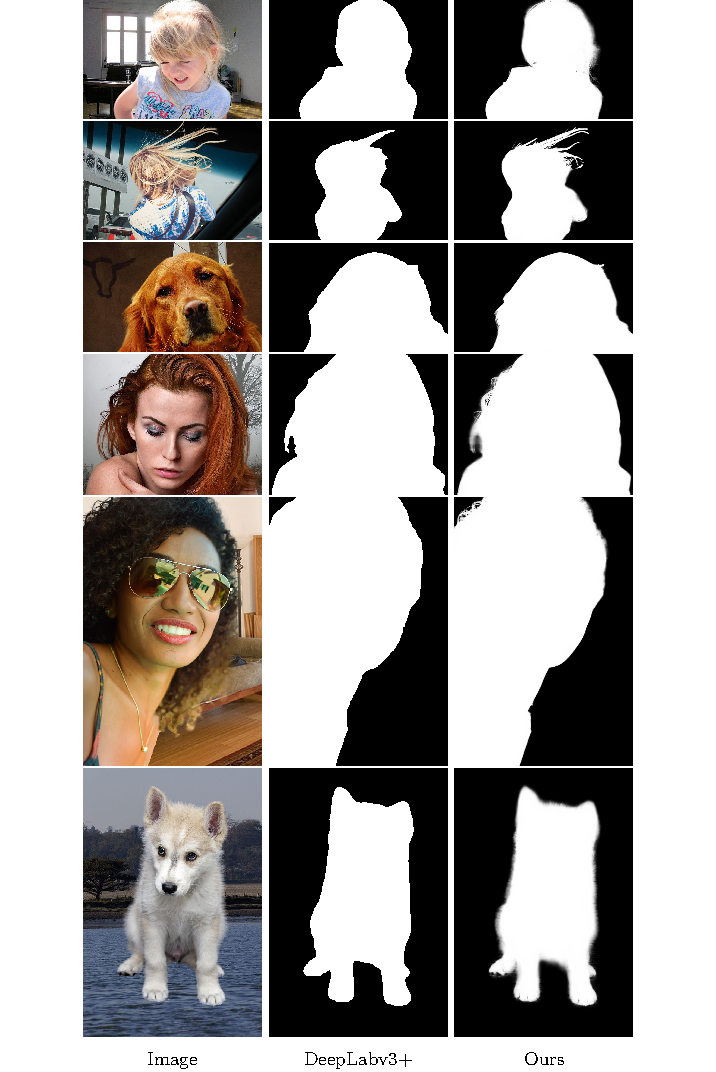
\includegraphics[width = 0.8\columnwidth]{chap6/adobe_deeplab.pdf}
	\bicaption{Composition-1k测试集中部分样本的抠图结果,分割蒙版由DeepLab v3+生成}{Results of samples from Composition-1k testing set. Masks are generated by DeepLab v3+}
	\label{fig6:adobe_deeplab}
\end{figure}
\section{本章小结}
在本章中,我们提出了一个借助引导滤波其中所隐含的梯度先验信息,以粗糙的弱标注分割结果替代trimap图的图像抠图方法。所提出的轻量级主干网络模型,使得该方法在移动设备上具有极高推理效率。此外,所提出的Gabor损失可以对抠图结果中的高频细节信息实现有效地监督。在两个测试数据集上的测试结果表明,所提出的方法对弱标注的分割蒙版输入具有一定的鲁棒性,同时在图像抠图任务中充分具有提取纹理细节的能力。